\documentclass[conference]{IEEEtran}
\usepackage{graphicx}
\usepackage{amsmath}
\usepackage{caption}
\usepackage{float}

% Title and author
\title{Performance of SPMV Calculation on GPU}
\author{Charlie Flux}

\begin{document}
\maketitle

\begin{abstract}
This paper investigates the performance of sparse matrix-vector multiplication (SPMV) on both CPUs and GPUs using the ELLPACK (ELL) \& CSR Compressed Spare Row (CSR) formats.
Both parallel methods were run on a GPU and CPU.
\end{abstract}

\section{Introduction}
The purpose of this experiment is to compare the performance of different matrix representations. Specifically, it examines how varying thread counts affect the performance of parallel sparse matrix-vector multiplication algorithms.
\section{Methodology}
2 Methods of storing matricies were used:
\begin{itemize}
    \item \textbf{ELLPACK (ELL)}
    \item \textbf{Compressed Sparse Row (CSR)} 
\end{itemize}

For experiments on the GPU, measuring time, thread counts \(T\) were chosen from the set:
    \[
    T = \{8, 12, 16, 24, 36, 48, 64, 72, 84, 96, 128, 256, 512, 1024\}
    \]
All experiments used the arguments the matricies provided by cant.mtx \& b.mtx files.
\subsection{Experimental Setup}
All tests were ran on Talepas. Experiments were repeated 20 times and the average was calculated for each experiment. \\
Data was filtered using the Interquartile Range Filter to remove points that do not lie between the first and third quartile as a consequence of the the unreliable data caused by the unlocked variable frequencies on Telepas.

\section{Results}

\subsection{ELLPACK Format}
I first implemented a naive kernel using minimal reduction techniques which performed poorly. 
This implementation contained a per thread processing technqiue with no load balancing and did not take advantage of shared memory.
Due to these design choices there is inefficient memory reads as each thread is reading data independantly leaving redundant memory accesses. \\
I then implemented a more complex kernel which made use of reduction techniques which can be seen in Figure \ref{fig:zoomed} by the 2x speedup in calculation times.
This optimized kernel leveraged shared memory to store partial sums, enabling threads within a block to collaborate on computing the sum for a row. 
The reduction phase utilized shared memory to perform partial sum reductions, significantly improving memory efficiency and overall performance. \\
Interestingly best performance for the improved kernel can be found at $\approx48$ threads whereas the best performance for the naive kernel is higher at $\approx72$ threads.
I belive the mainly is due to the added overhead of the complex kernel from thread synchronisation during the reduction phase.
\begin{figure}[H]
    \centering
    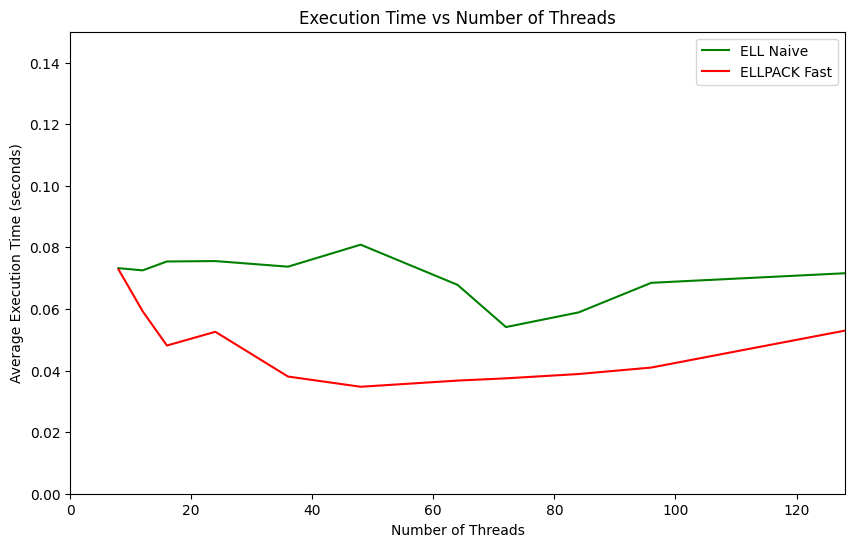
\includegraphics[width=0.45\textwidth]{../img/ellpackzoomed.png}
    \caption{SPMV GPU Implementations}
    \label{fig:zoomed}
\end{figure}

\subsection{CSR Format}
I next completed a kernel for the CSR format which saw performance better than the naive ELLPACK kernel but worse than the optimised ELLPACK kernel.
The main disadvantage of the CSR format which the ELLPACK aims to improve is the irregular memory access pattern which could be a reason why the ELLPACK performs more efficiently.
The CSR format also is most efficient at $\approx72$ threads which could be due to the similar reduction pattern that is implemented in the naive ELLPACK kernel.  
\begin{figure}[H]
    \centering
    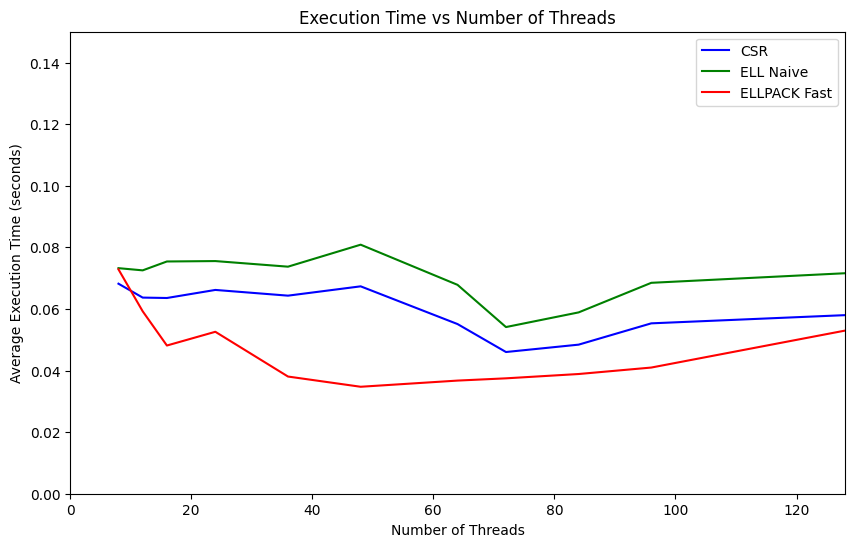
\includegraphics[width=0.45\textwidth]{../img/gpuzoomed.png}
    \caption{CSR implementation}
    \label{fig:parallel}
\end{figure}

\subsection{Increasing the Number of Threads}
Increasing the number of threads shows that the ELLPACK format does not scale well with threads whereas, the CSR format handles the increased number of threads well.
The naive approach performs better than the complex approach when the threads are increased. 
This could be from the shared memory usage constraints during the reduction.
With more threads, the shared memory per block increases and if this exceeds the limit for the GPU then this reduces the number of active thread blocks.
An increase in threads also sees an increase in the fraction of inactive threads during the reduction phase resulting in an underutilisation of the GPU.

The complex kernel relies on thread synchronization, which introduces a waiting phase as all threads must reach the synchronization point before proceeding. As the number of threads increases, this waiting time grows because threads performing more extensive or slower tasks can delay the others. This leads to higher overhead and reduces overall performance efficiency.
\begin{figure}[H]
    \centering
    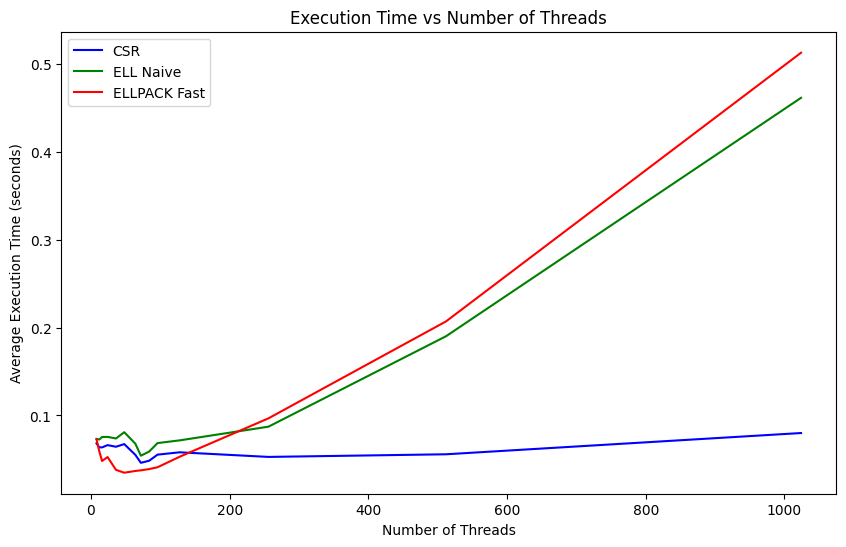
\includegraphics[width=0.45\textwidth]{../img/gpu.png}
    \caption{COO to CSR Conversion}
    \label{fig:conversion}
\end{figure}

\section{Conclusion}
This experiment compared the performance of SPMV calculations on GPUs using the ELLPACK and CSR formats.
The CSR format, while not as efficient, outperformed the ELLPACK format as the threads increased above $\approx128$ by removing padding overhead and utilising its compact format.
However, the ELLPACK performs the best at lower thread counts ($<128$) due its optimised memory access patterns.
\end{document}
